\documentclass[11pt,twoside,a4paper]{report}
\usepackage{appendix}
\usepackage{geometry}
\usepackage{graphicx}
\usepackage{pdfpages}

% set the default, standard, geometry
\geometry{left=25mm, right=25mm, top=25mm, bottom=25mm}

\setlength{\parskip}{\baselineskip}
\clubpenalty10000
\hyphenpenalty10000
\widowpenalty10000

\begin{document}

\title{ID2216 Developing Mobile Applications\\Project Report}
\author{Rafael Aldana (rafaelap@kth.se)\\Vincent Delitz (delitz@kth.se)\\Ruth Eriksson (ruthe@kth.se)}
\date{\today}
\maketitle

\newcommand{\webOrNative}{Web~}

\begin{abstract}
During the course, we have worked in team to propose, build, and document a mobile app. We have developed a functional \webOrNative application that addresses an interesting and relevant area we have identified. This report describes step-by-step how we designed the mobile application.
\end{abstract}

\tableofcontents
\thispagestyle{empty}

\listoffigures
\thispagestyle{empty}

%\listoftables

\renewcommand{\chaptername}{Assignment}
\setcounter{chapter}{0}
\chapter{Project proposal}
\setcounter{page}{1}

\section{Brainstorming}

At the very beginning, we started to think about general hypes and most current usages of mobile applications and tried to define some fields that were interesting to do a more detailed research. Some of these fields were mobility, travel, IoT, sharing, collaboration, big data, and digitalization. Of course, this is still too much to get any detailed results or to find a concrete idea for a mobile application.

So the next step was to think of problems that we faced on our own in daily life, that could be solved by a suitable application. Some outcomes of this are listed below:

\begin{itemize}
	\item Since it is often very hard to find a decent present for someone's birthday or for Christmas, it would be very useful to have an app that suggests suitable presents. This could be done based on the presents or wishes someone has submitted, so that others can see what they could go for a gift.
	\item Another idea was to build a portal where people who have to stay home because they are too old, disabled, or injured, can place a groceries list so that others can buy those and deliver them for a small fee. Both parties would benefit from it since old, disabled, injured people get their groceries and students, for instance, who do the groceries could earn little money and do social work.
	\item Our third idea for a useful application was based on a personal experience of a team member. It is quite common in Stockholm to buy or sell SL cards for public transport from or to other people, and there are a lot of offers in Facebook groups or other websites on the Internet, but they are not standardized, and it is sometimes quite hard to find a suitable ticket. A solution for this could be a portal where people can offer and search for SL cards that is easy to use and standardized. All three of us agreed that this idea is worth to spend more time on a deeper research.
\end{itemize}

\section{Observation-based field study}

After we agreed on a rough idea for our application, we decided to research our application domain, travel and mobility, in more depth. So we tried to observe if and how people use mobile applications while they are travelling by public transport.

We chose to observe this behaviour at both Kista and Stockholm Central station. Additionally, we also put focus on buying SL cards and how people use it at the station. Our observations are gathered below:

\begin{itemize}
	\item Most of people use their smartphone a lot, while waiting for a train or walking to the correct line. Unfortunately, it is quite hard to see which exact kind of apps they are using, but many of them listened to music, seemed to play games or read the news.
	\item Many people also use their smartphone to check their route and the time schedule for the trains.
	\item Sometimes there are long queues at the counters if you want to buy a SL card or recharge it, while the vending machines are not used.
	\item Some people try to cheat. They do not buy a ticket and just go through the gate after someone who opened it by validating the SL card.
	\item Many people communicate with others through messaging apps or they are just calling someone.
\end{itemize}

After observing the public transport system live, we changed our focus to the Internet and how people try to sell and buy SL cards here. Of course you can buy tickets on the official website of the public transport system, but there are also other ways to buy tickets.

We also found a lot of Facebook groups where people were posting about SL cards. Each of these offers had a tentative price for the card given its expiration date. Other information, like where to pick the card up or if it is a special card for students, was often missing. Furthermore, there was no standardization for the offers and each had its own format.

We also found offers for SL cards on websites such as www.blocket.se. However, they were still not standardized as it happens in the Facebook groups. Moreover, from some of the posts you could not clearly recognize if someone was offering or searching for a card. On top of that, it took sometimes quite a while to find an offer for a SL card and looking for a specific period of validity was even much harder.

Then, we had found a problem that we wanted to solve with our mobile app, but we were still not sure what potential users could think about it as a good solution. So we conducted some interviews with friends and family members in order to get their opinion for our idea, get possible new features, and if this app could help them.

Therefore, we created a set of questions that we asked each participant. These questions started very general about the public transport system in Stockholm and then we narrowed it down to the trade of SL cards. The majority of our interview participants lives permanently in Stockholm, but we also questioned a tourist in order to also cover this potential user group. A description of our questions and a summary of the answers are gathered below:

\begin{itemize}
	\item \textbf{\textit{How often do you use the public transport system?}} Most of the people we questioned and who live in Stockholm use the public transport system almost daily. They use it to get to the university, to their work and also for leisure time activities. Mostly, they take the metro and commuter trains, but also buses and trams. On the contrary, the person who does not live permanently in Stockholm but is every four to five weeks in the city uses the public transport normally on the weekends or in the holidays.
	\item \textbf{\textit{Do you have a 30-days or 90-days ticket?}} People who live regularly in Stockholm usually have a 90-days pass, unless they plan to be out of the city. Tourists don't usually buy such a ticket, they take a 3-day pass or, if their stay is longer, a 7-day pass instead.
	\item \textbf{\textit{If you do not have a 30/90-days ticket, do you pay per ride?}} We found out that if someone has a 30/90-days ticket, he does not pay per ride of course, but some tourists who stay in Stockholm for maybe four or five days buy a 3-day pass, and on the other two days they pay per ride. If they foresee they need to travel often on those days, they just buy a 7-days pass instead, since this is cheaper than two 3-days passes and they just do not make the most of the last days of the 7-days period.
	\item \textbf{\textit{What do you think about the prices for public transport in Stockholm?}} The general participants' perception of the prices was that it is quite high, especially if you are a student, even though you get a discount. In other European capitals you pay way less than in Stockholm. But some others answered that the reduced price is fair, since you can go anywhere in the city and take any means of transport. If you do not get a discount on the fares, it is really expensive, stated one of the participants. Since we can do nothing about the prices, our point is to solve the problematic of the fact that short period passes (3/7-days) are very expensive proportionally compared to 30-days tickets.
	\item \textbf{\textit{Do you get any discount on the fares?}} Since we mainly questioned students, the majority got discounted fares for the tickets, but there were also people who had to pay the regular price.
	\item \textbf{\textit{Have you ever searched for a SL card on the Internet? If yes, how did you find it? Was it easy or laborious?}} Some of the participants said that they have not searched specifically for a SL card, but they have seen offers in Facebook groups. If one had searched for a card, he said that it is really laborious to find a suitable ticket, since the offers are spread over different portals and groups, and if you found a suitable ticket, it is often really cumbersome to retrieve it from the seller and to communicate with the seller about the details.
	\item \textbf{\textit{What do you think about our idea for a platform to trade SL cards? Do you have any suggestions or wishes or is there anything else you want to mention?}} Some said that it would be really useful for them if they can rent out their SL cards while they are on vacation. So they would get a little compensation for the time they are not in town, but still could purchase a 90-day pass. Additionally, all agreed that both the seller and the buyer would benefit from this app, the buyer by getting cheaper and more flexible public transport tickets and the seller by getting money back if he does not need the SL card anymore.
\end{itemize}

\section{Proposal}

After all these findings, we decided to build an application that provides its users with the opportunity to offer and search for SL cards. These SL cards have to be, of course, not registered at the carrier in order to make them transferable.

This app will be as easy-to-use as possible with a very simple and clear user interface. Within a few steps each user should be able to find or post what he wants. The offers will be kept in a standardized format and users will find all relevant information about a given offer in the app. Furthermore, users should be able to get notified if someone has posted an offer for a SL card that fits to a desired pattern.

Besides simple selling or buying, users should also have the opportunity to rent and rent out their SL cards. Moreover, the user will see directly in the app where they can pick up the SL card, whether the prices and the period of time are negotiable and contact information will also be visible in the app.

This app will be improved step-by-step with a lot of feedback loops to make it as user-friendly as possible and to adapt to changed requirements from the users. We will start with a paper prototype for a rough understanding, moving onto a web app prototype and then to a native app prototype until we have a working solution.

\chapter{WebApp Prototype}

Once we agreed to develop an application that helps users to find and offer SL cards in the previous assignment, we focused on creating first prototypes and getting a preliminary structure for the application. Therefore, we created a paper-based prototype and collected feedback from potential users and friends.

Based on this, we aimed to create a site map of the different layouts of our application and how the user navigates through our app by creating a clickstream. Additionally, we developed a new digital "paper-based" protoype of our app by using the online tool Balsamiq.

\section{Paper prototype}

The very first step for creating the paper-based prototype was to think about which basic layouts and functionalities does our user need. So, we took a paper and a pencil and started drawing the main views. We discussed a lot about which features are really necessary for the first version of our app, since it must be as slim and lean as possible.

Furthermore, we tried to incorporate basic design principles of Android applications, so that the user will easily adapt to the usage of our application. This was carried out by using common design patterns of Android apps as well as a really clear structure.

The outcome was a paper prototype based on eight different views, all of which had a quite similiar design and an easy usability from our point of view. See figures~\ref{figure:paper-prototype-1} and~\ref{figure:paper-prototype-2} on pages~\pageref{figure:paper-prototype-1} and~\pageref{figure:paper-prototype-2} respectively.

\section{Site map}

After finalizing the paper-based prototype, we showed it to friends and other potential users in order to gather their impression and feedback. All in all, they liked the first prototype quite much, since it was also very simple and good in their opinion. Nevertheless, some also showed us that we missed little things or could improve the prototype at certain points. Some of the major feedback points we discovered are listed below:

\begin{itemize}

\item It would be nice to have start screen with the logo of our app, before reaching the home screen.

\item There should be a "Log out" button in the swipe menu on the left.

\item It would be cool to have settings screen, where you can define the date/time format and the displayed currency.

\item The offer details must definitely contain the user behind the offer and his contact details. Furthermore, it would be good to see how long he has been registered in the app.

\item A support tab in the swipe menu would also be nice, in case there are any questions or feedback for us.

\item As a matter of privacy, there should be an option if people searching for a SL card can see the mobile number of the seller or not. I think if someone sees the email address, this is fine, but the mobile number is quite sensitive.

\item It would be cool to have, maybe in a later stage, also an integrated chat system to contact the seller of a card.

\item It would be nice to see a suggested price for the given validity period.

\item Be sure to implement the insertion of the date with the popup calendar.

\item Why so much data at login? Would not it be enough with username and password to log in?

\item It would be nice to change free text for extra information or comment or something more understandable.

\item Credit is not very clear and could be confuse with Price. What about Saldo?

\item It would be good to change Pick Up Place for Pick Up Station, if that is restricted to stations, we ensure that the buyer has a chance to check the validity of the card. In addition, it feels safer to meet that way.

\end{itemize}

Next, we discussed which of the feedback will be implemented in the next prototype and which not. For this new prototype we created the site map that displays all layouts of our app structuredly. See figure~\ref{figure:site-map} on page~\pageref{figure:site-map}.

\section{Balsamiq prototype}

With the existing site map, it was time to create a new prototype. This time not with a pen and paper, but with the online tool Balsamiq. This tool was also already used to draw the site map chart. Balsamiq is a quite handy and useful tool that allows you to develop prototypes for apps and other software in a very fast way by providing with drag-and-drop functionality.

So, we created for each screen at least one wireframe in order to make the prototype as real as possible. By using the framework of Balsamiq, we could
insert a lot of real Android API components, such as the map functionality.

\section{Clickstream}

After finishing the Balsamiq prototype, we created additionally a clickstream of the current prototype that shows how the user later will navigate through the app. See figure~\ref{figure:clickstream} on page~\pageref{figure:clickstream}.

\section{WebApp prototype}

Based on the feedback we received for the previous prototypes, we created a Webapp prototype. Therefore, we decided to use the Bootstrap framework, since it is quite easy to use for beginners and the results looked pretty reasonable. For distributed developing, we created a git repository to share the code and used Sourcetree to handle the different versions. See figures from~\ref{figure:start-page} to~\ref{figure:settings-page} in appendix~\ref{webapp-prototype-appendix}.

\begin{appendices}

\chapter{Paper prototype figures}
\thispagestyle{empty}
\newpage

\begin{figure}
	\centering
	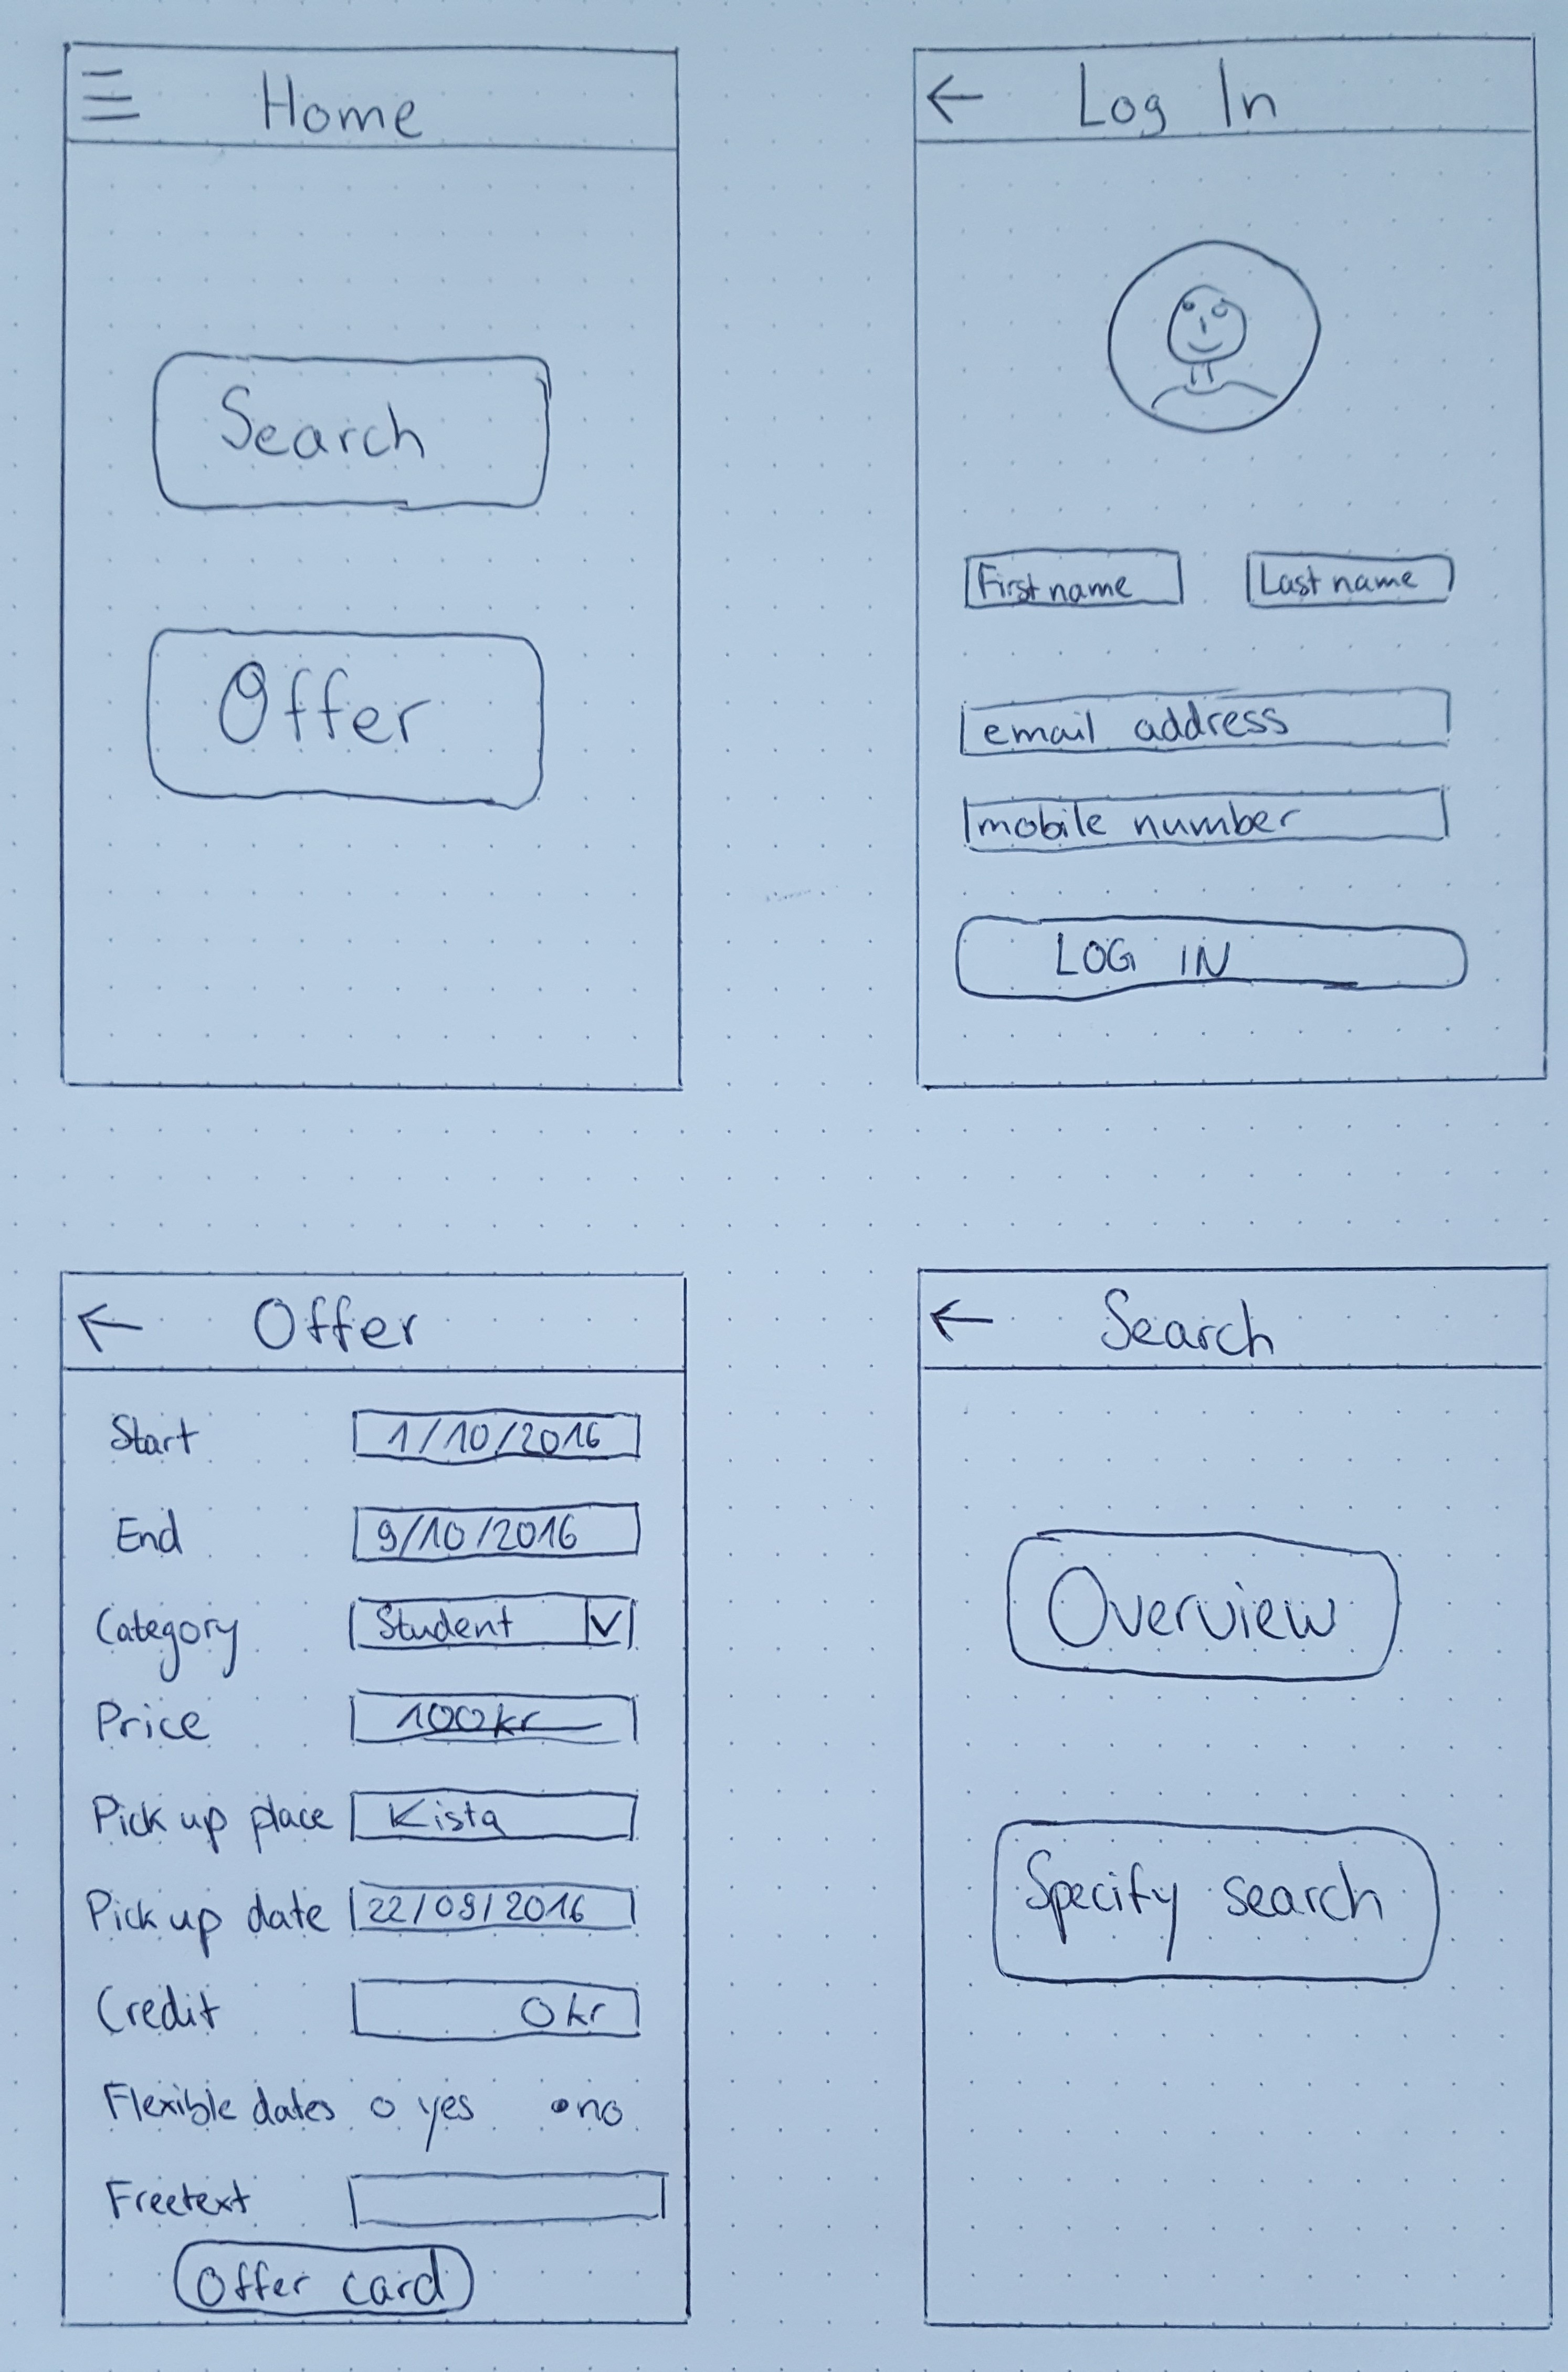
\includegraphics[width=\textwidth]{jpg/paper-prototype-1.jpg}
	\caption{Paper prototype figures}
	\label{figure:paper-prototype-1}
\end{figure}

\begin{figure}
	\centering
	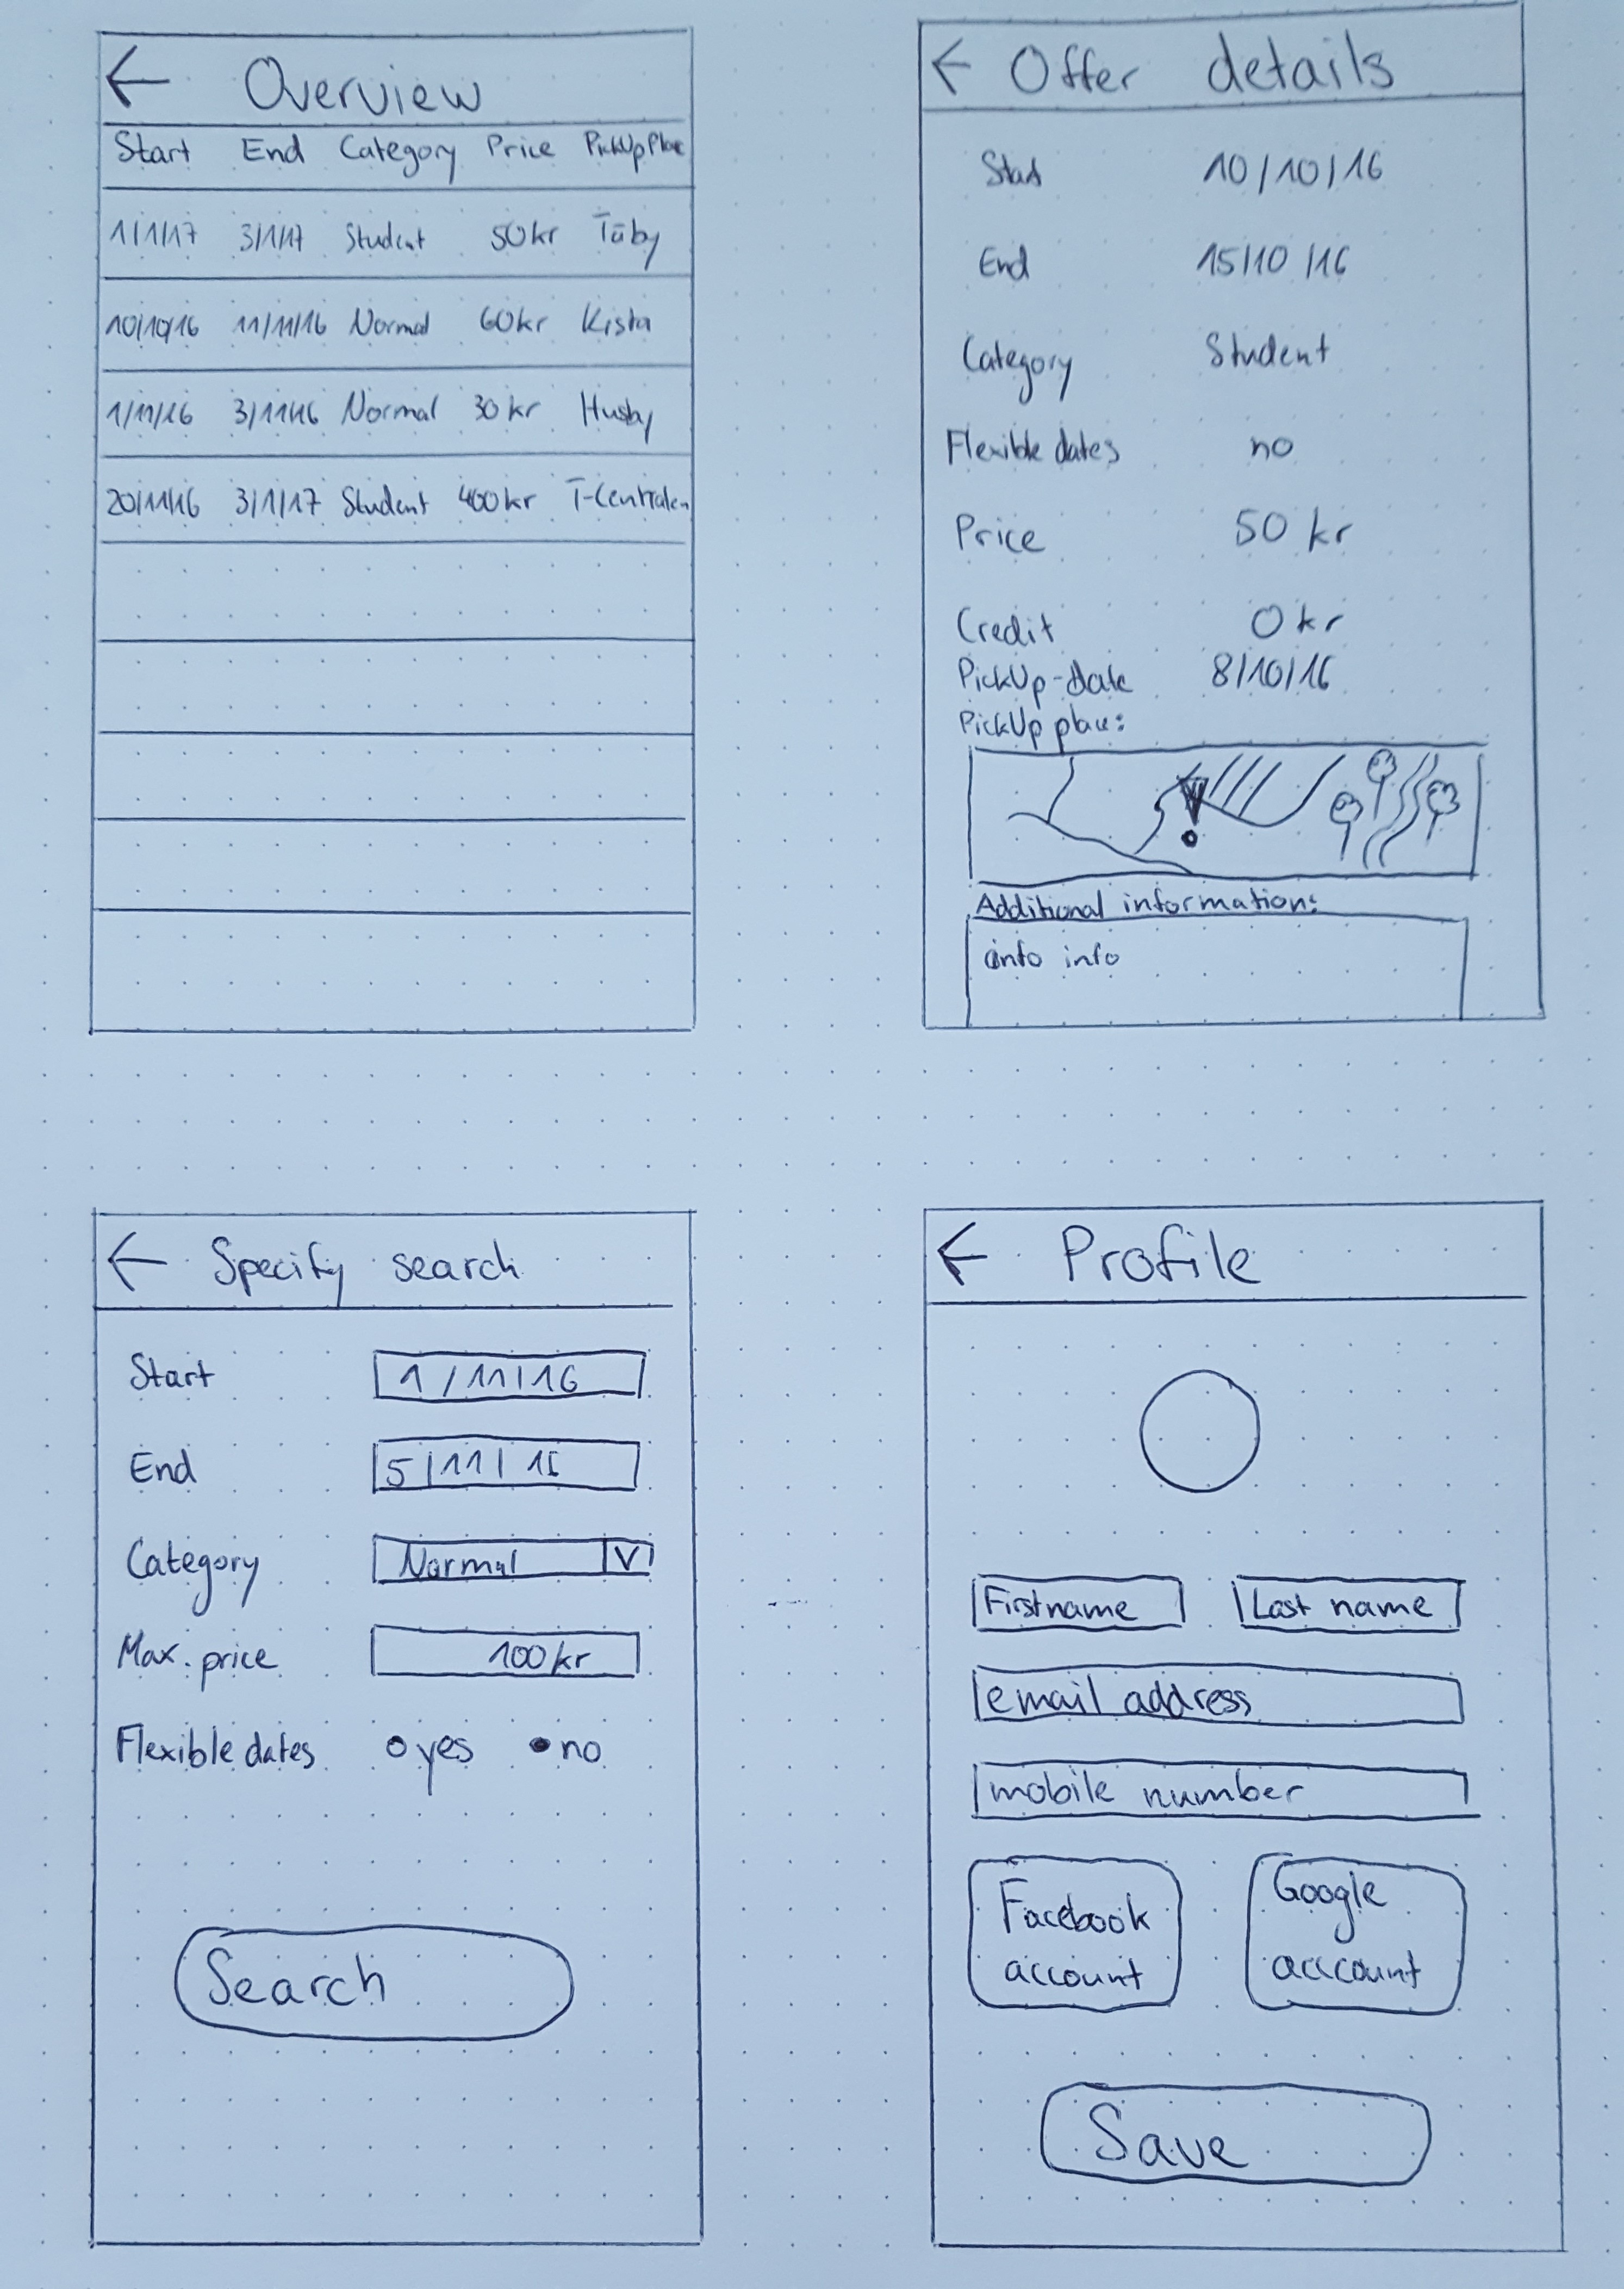
\includegraphics[width=\textwidth]{jpg/paper-prototype-2.jpg}
	\caption{Paper prototype}
	\label{figure:paper-prototype-2}
\end{figure}

\chapter{Site map and clickstream figures}
\thispagestyle{empty}
\newpage

\begin{figure}
	\centering
	\includegraphics[page=9,width=\textwidth]{pdf/balsamiq.pdf}
	\caption{Site map}
	\label{figure:site-map}
\end{figure}

\begin{figure}
	\centering
	\includegraphics[page=10,width=\textwidth]{pdf/balsamiq.pdf}
	\caption{Clickstream}
	\label{figure:clickstream}
\end{figure}

\chapter{WebApp prototype figures}
\label{webapp-prototype-appendix}
\thispagestyle{empty}
\newpage

\begin{figure}
	\centering
	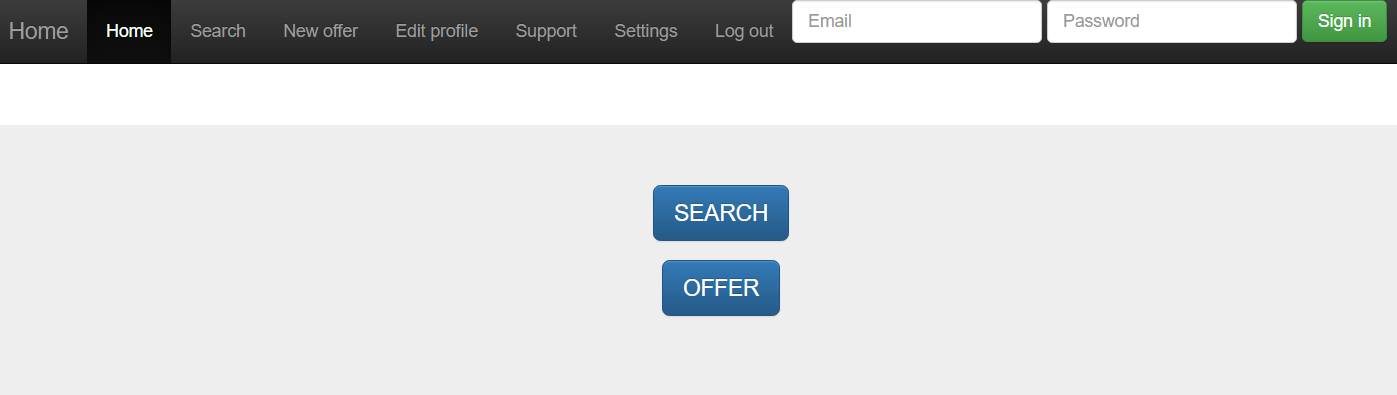
\includegraphics[width=\textwidth]{png/webapp-start.png}
	\caption{Start page}
	\label{figure:start-page}
\end{figure}

\begin{figure}
	\centering
	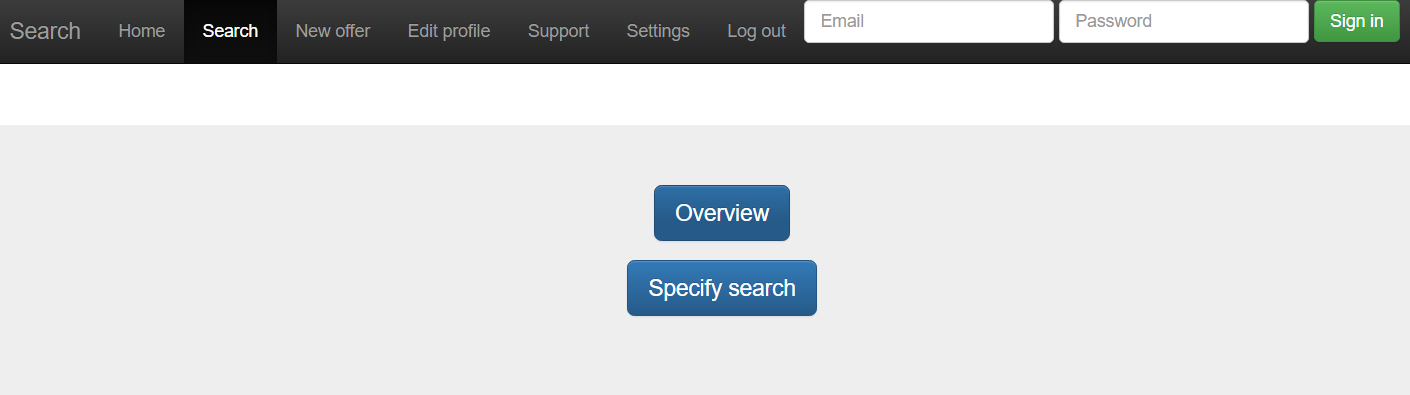
\includegraphics[width=\textwidth]{png/webapp-search.png}
	\caption{Search page}
	\label{figure:search-page}
\end{figure}

\begin{figure}
	\centering
	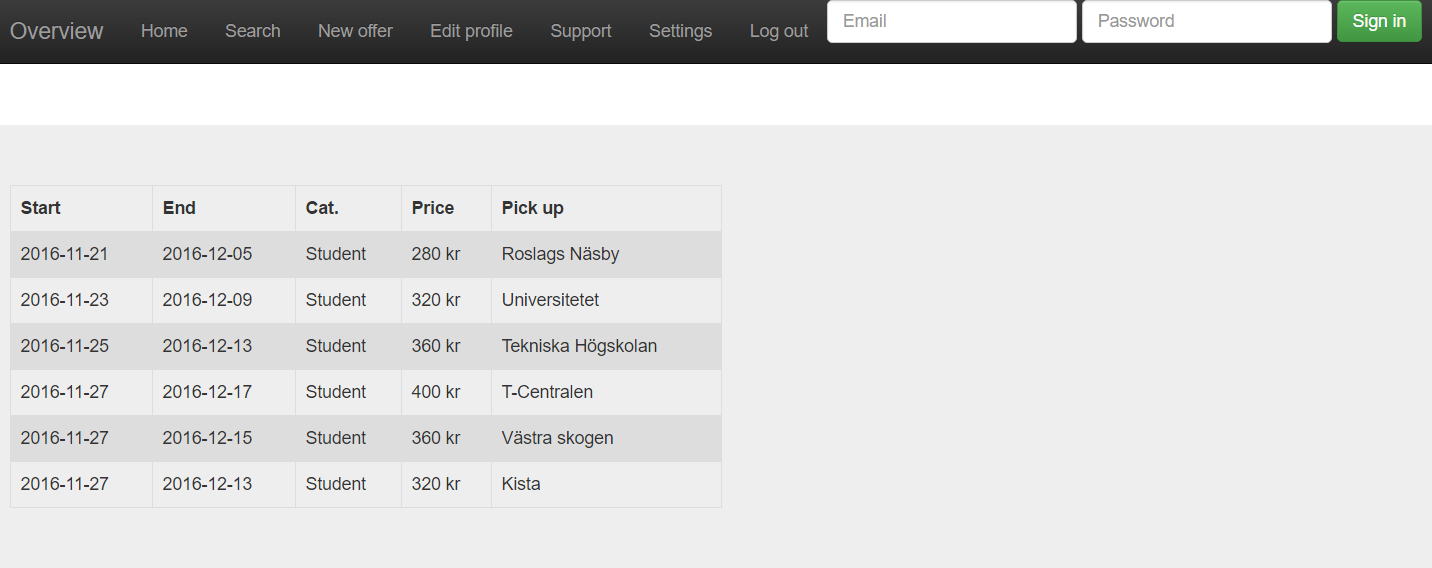
\includegraphics[width=\textwidth]{png/webapp-overview.png}
	\caption{Overview page}
	\label{figure:overview-page}
\end{figure}

\begin{figure}
	\centering
	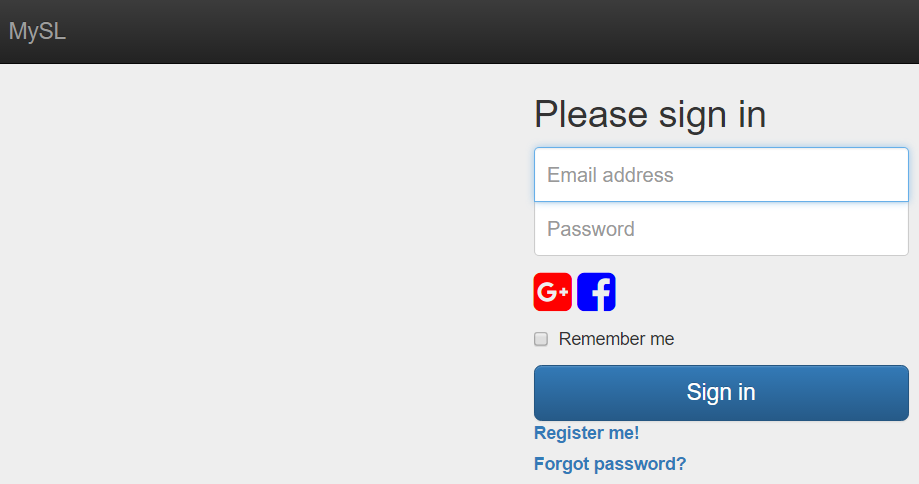
\includegraphics[width=\textwidth]{png/webapp-login.png}
	\caption{Login page}
	\label{figure:login-page}
\end{figure}

\begin{figure}
	\centering
	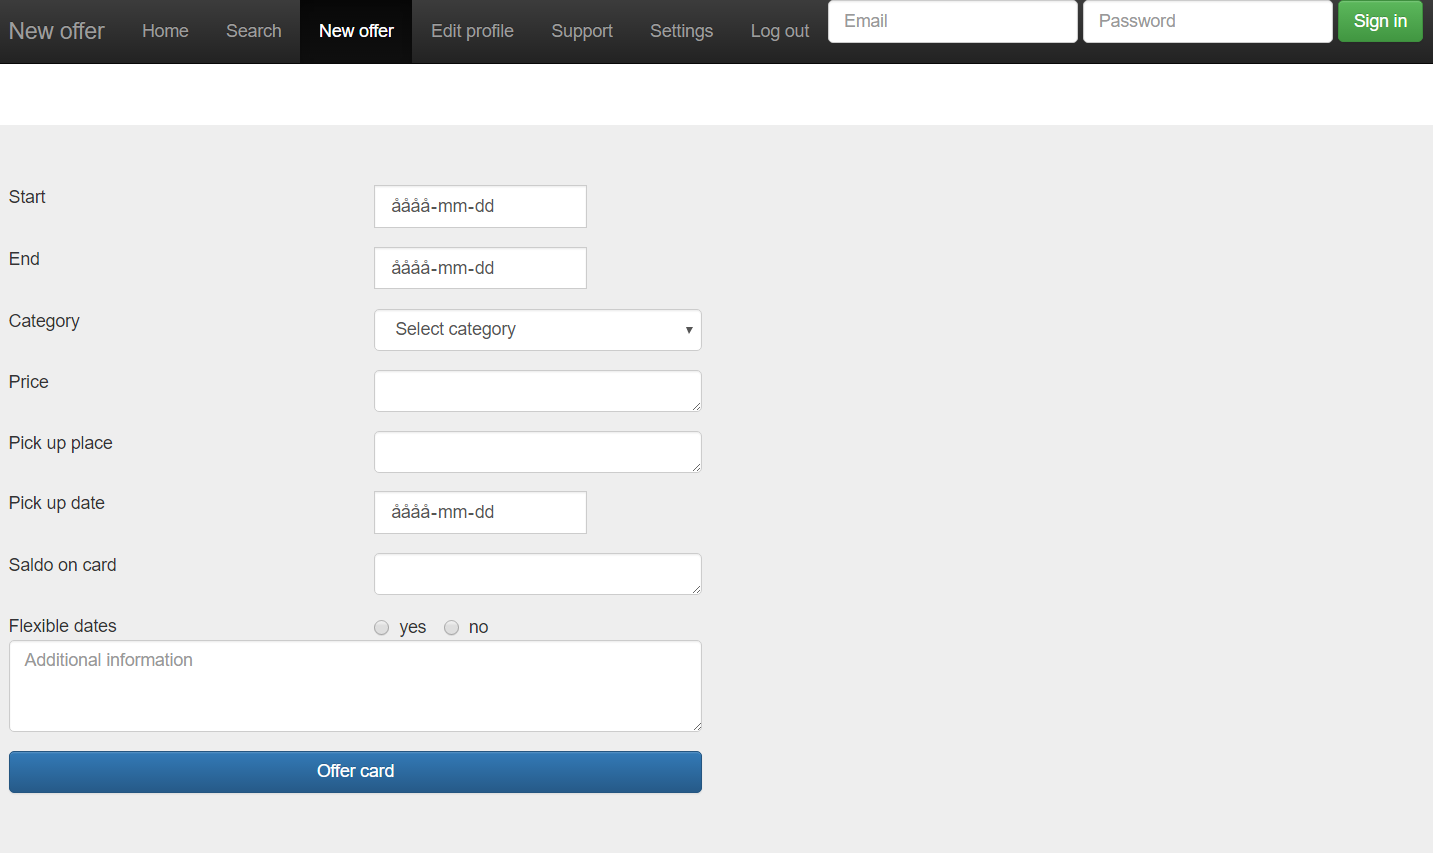
\includegraphics[width=\textwidth]{png/webapp-newoffer.png}
	\caption{New offer page}
	\label{figure:new-offer-page}
\end{figure}

\begin{figure}
	\centering
	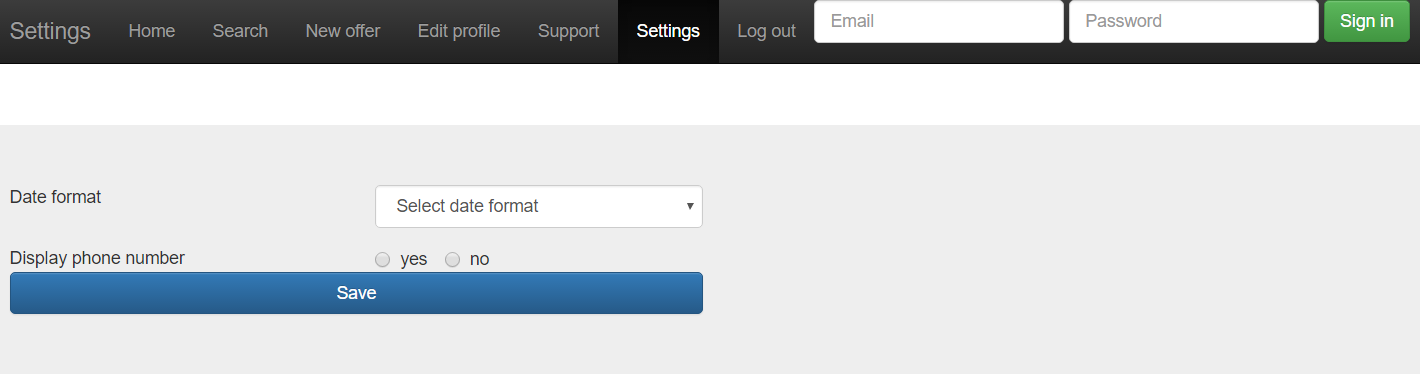
\includegraphics[width=\textwidth]{png/webapp-settings.png}
	\caption{Settings page}
	\label{figure:settings-page}
\end{figure}

\end{appendices}

\end{document}